% Build the vector architecture figure with:
%   dot -Tpdf architecture.dot -o architecture.pdf
% Build the paper with:
%   latexmk -pdf -interaction=nonstopmode main.tex
\documentclass[sigconf,nonacm]{acmart}
\usepackage{placeins}
\settopmatter{printacmref=false,printfolios=true}
\setlength{\emergencystretch}{1em}

\begin{document}
\title{SQLolla: Bounded Evidence Review for PostgreSQL Queries}
\author{Claudius G.P.T. Slopius}
\affiliation{%
  \institution{University of Wild Chicken}
  \city{}
  \country{}
}
\email{slop@uwc.edu.bi}
\author{Saya de las Geminis}
\affiliation{%
  \institution{University of Wild Chicken}
  \city{}
  \country{}
}
\email{saya@uwc.edu.bi}

\begin{abstract}
SQLolla compiles supported PostgreSQL statements to typed relational algebra, searches finite models with Alloy, and stores replayed examples and counterexamples. Reviewers label concrete behavior to preserve or exclude during query revision. A deterministic gate replays the labeled cases and checks the original bounded assertion before a candidate can be adopted. Evaluation covers 276 parser exports, 552 recorded PostgreSQL observations, and 3,511 fresh comparisons on the native relational fragment. The browser workbench was exercised on Windows, Ubuntu under WSL2, Docker, and the deployed website. Starting from an empty workbench, a live provider request produced a locally compiled inventory model. A separate browser replay edited the SQL, preserved the model, and found a counterexample to the selected row limit.
\end{abstract}

\keywords{PostgreSQL, relational algebra, Alloy, bounded model checking, counterexamples, query refinement}
\maketitle

\section{Introduction}
A business query can return another tenant's rows while remaining syntactically valid and well typed. SQL review often leaves the database input that triggers the behavior implicit. SQLolla accepts a query, a schema, a finite domain, and an explicit rule. A check returns a replayed counterexample or a search status with its bounds. Reviewers can inspect the input and output rows together with the canonical SQL, relational algebra (RA), and Alloy model.

We distinguish three evaluation questions. Parser coverage measures whether a record can be exported as structured syntax. Semantic replay measures agreement with a stated PostgreSQL observation under its supplied context. Refinement measures whether a candidate retains labeled behaviors and satisfies the original assertion within the original bounds. These questions use distinct oracles and denominators.

\begin{figure*}[t]
  \centering
  \includegraphics[width=.98\textwidth]{architecture.pdf}
  \caption{SQLolla separates deterministic analysis and replay from optional provider assistance. PostgreSQL serves as a test oracle, and Lean specifies interface contracts.}
  \Description{Architecture diagram. The browser sends SQL and a bounded rule to the Rust host. SQLeanParser exports a syntax tree. Rust binds it into typed relational algebra and produces an Alloy model. The Java bridge sends that model to Alloy. Rust replays the result and saves evidence. The browser can request a model or SQL draft and can ask OpenAI to explain an archived case. Lean and PostgreSQL connect through development checks.}
  \label{fig:architecture}
\end{figure*}

\section{Architecture and evidence}
Figure~\ref{fig:architecture} follows the request from the workbench to the archive. The pinned SQLeanParser adapter exports syntax. Rust binds relation names and typed parameters against a closed catalog, lowers the statement to typed RA, and emits the Alloy source. The Java~17 bridge calls the Alloy API. The encoded model distinguishes satisfiable assumptions from the assertion being checked. A satisfiable counterexample is decoded and replayed before the host presents it to a reviewer.

Codd's relational model provides the algebraic setting~\cite{codd1970}. Jackson describes translating constrained relational models into bounded SAT problems~\cite{jackson2000}. SQLolla follows this bounded search approach and preserves bag multiplicity, typed nulls, and ordered output positions. It records observable errors and effects when the admitted profile supports them.

The native relational profile compares a separately encoded Alloy result with the Rust interpreter. A wider profile encodes a complete table of finite outcomes produced by the interpreter. Its Alloy check exercises outcome selection and replay. Independent PostgreSQL comparisons are needed to assess the evaluator's SQL semantics. An inconsistent assumption set, timeout, coverage failure, or truncated search does not establish a bounded pass.

\section{Build with AI}
The workbench opens with an empty query and catalog. Users can declare a model themselves or describe it through Build with AI. A new-model request sends the description with explicit consent. Drafting SQL for an existing model also sends schema declarations and numbered parameter types. The host checks the proposed SQL with the local compiler. The user selects the proposal before it becomes the editable workbench request and runs the bounded analysis explicitly.

In a live bring-your-own-token (BYOT) trial on \texttt{d71e8cf}, the user described an \texttt{inventory} table with two non-null \texttt{int32} columns, \texttt{item\_id} and \texttt{units}, and at most one row. The finite domain contained 0, 1, and 5. The rule allowed at most zero output rows. The reported proposal selected both columns from \texttt{inventory} and passed the compiler check. In a separate Chrome replay on the same deployment, we staged the model and submitted the following edit.
\begin{verbatim}
SELECT item_id, units
FROM inventory
WHERE units = 5
\end{verbatim}
Alloy found an input with \texttt{item\_id = 5} and \texttt{units = 5}. The edited query returned that row, violating the zero-row rule, and Rust confirmed the result by replay. Figure~\ref{fig:workbench} shows the blank composer and the replayed witness.

\section{Review and refinement}
Each case fixes an input $d$ and an observed behavior $b$. Write $O(q,d)$ for the complete set of modeled outcomes for candidate $q$ at that input. A Yes case requires $b \in O(q,d)$. A No case requires $b \notin O(q,d)$. Unsure retains a review decision without a replay obligation. The checker requires at least one active Yes or No, a compatible review basis, and a clean check of the original assertion within the original bounds. A candidate can become the next SQL draft only after the user chooses to adopt it. Editing the prompt or labels invalidates earlier adoption eligibility.

This loop resembles counterexample-guided synthesis~\cite{solar2008}. Here the candidate can come from a reviewer or a model, and the admissible checks are bounded. We make no convergence guarantee. Cosette addresses SQL equivalence and counterexamples~\cite{chu2017}. SQLolla's evidence references identify concrete case facts. Why- and where-provenance provide a broader framework for tracing outputs~\cite{buneman2001}.

\section{Redacted assistance}
Assistance is optional. The first-visit prompt offers setup and a skip action. A provider key stays in tab memory and accompanies only an explicit request. The host reloads the selected instance from its archive, builds the packet, and checks the returned identities and fact citations. Model prose remains untrusted. The source triple, rule value, parameters, domain values, and row payloads stay local in redacted mode. The user's optional question is transmitted as written.

In the live deployment, a redacted answer identified one input-row occurrence and one output-row occurrence. The user reported that this gave no useful reason for the violation. The revised projection supplies the verified rule outcome. For a required-value rule it gives the output column position and a citation to a row whose typed value differs from the requirement. For a forbidden-value rule it supplies a matching witness. Row-limit and execution-error checks disclose their verified outcome without the original rule constant or error text. The packet keeps the decisive row within the fact budget even when earlier input occurrences fill it. The instructions ask the model to explain the mismatch first and separate an inspection step from a proved cause.

The Lean contract formalizes the projection from an approved observation with private payload held separately. Equality of the approved observation suffices for equality of its projection. The contract also requires citations to resolve within the selected instance view. Lean checks these statements and their admitted foundations~\cite{lean2021}. Tests exercise typed nulls, duplicate rows, missing violations, redaction, and a witness beyond the normal fact budget. In a live trial of the revised deployment, a user-provided transcript identified a required-value mismatch at output position two and cited the offending row. The answer suggested checking the expression that produced that position and the expected value. It repeated the scope limits and left the cause undetermined. In a separate production browser test, a controlled response verified that both the returned-row and input-row citations open the matching facts from a fresh replay.

\begin{table}[t]
  \caption{Evaluation counts by validation boundary.}
  \label{tab:checks}
  \centering
  \small
  \begin{tabular}{@{}lr@{}}
    \toprule
    Gate & Observed \\
    \midrule
    SQLeanParser records exported & 276/276 \\
    Distinct SQL texts & 260 \\
    Recorded PostgreSQL observations & 552/552 \\
    Fresh native comparisons & 3,511/3,511 \\
    Fresh industrial comparisons & 24/24 \\
    Frontend unit tests & 84/84 \\
    \bottomrule
  \end{tabular}
\end{table}

\begin{figure*}[t]
  \centering
  \begin{minipage}[c]{.30\textwidth}
    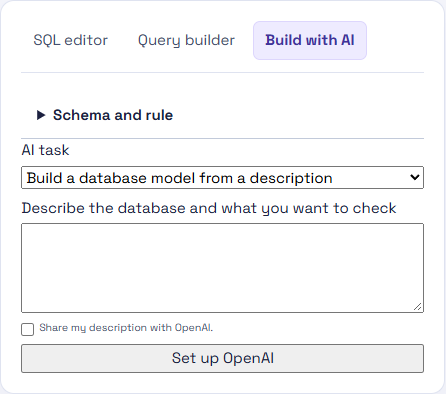
\includegraphics[width=\linewidth]{blank-workbench.png}
  \end{minipage}\hfill
  \begin{minipage}[c]{.66\textwidth}
    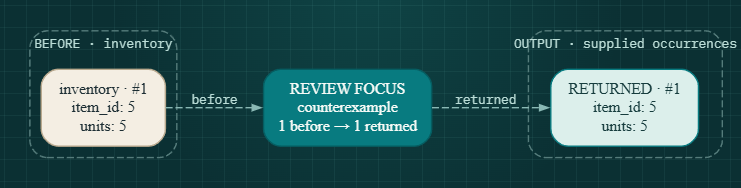
\includegraphics[width=\linewidth]{inventory-witness.png}
  \end{minipage}
  \caption{Build with AI on the blank production workbench (left) and the counterexample from a separate production replay of the edited inventory query (right). The edited query returned one row with \texttt{units = 5}.}
  \Description{The left image shows an empty description field and the option to build a database model. The right image shows an input inventory row with item ID and units both equal to 5, and the same values in the returned row.}
  \label{fig:workbench}
\end{figure*}

\section{Evaluation and deployment}
Table~\ref{tab:checks} summarizes the checks. The industrial ledger retains the supplied context for every SQL record, including driver expansion, bindings, and expected errors. The full ledger uses retained PostgreSQL outcomes. The independent PostgreSQL~16.16 cluster provided the fresh comparisons. Pivoted query synthesis illustrates the use of a separately justified test oracle~\cite{rigger2020}. Our comparisons instead use the actual PostgreSQL behaviors for the stated inputs and contexts. The refinement regression also exercises unordered \texttt{LIMIT} alternatives, duplicate occurrences, and expected PostgreSQL errors.

The \href{https://github.com/University-of-Wild-Chicken/SQLolla/actions/runs/43723047506}{hosted Windows run} passed the Lean audit, parser exports, PostgreSQL and Alloy replays, IIS archive verification, and Chrome against the extracted package. Browser checks cover the builder handoff, stage and copy actions, Graphviz, case reopening and Next, the review bins, and the first-visit and credential controls. Cloudflare Access initially gated the deployment~\cite{cloudflareaccess}. The inventory trial exercised the provider request through the deployed proxy. The separate browser replay verified that the edited SQL reached the host with its original finite model and that the workbench opened the replay-confirmed witness.

The private IIS and Linux packages include the host, parser, Java runtime, Alloy bridge, and static assets. Chrome passed against the Linux archive in Docker on Ubuntu under WSL2. The image requests \texttt{SIGINT} on stop~\cite{dockerstop}. The process exited with code zero, and a restarted container reopened the identical saved case from the named volume. Archive provenance binds compiler bytes. A platform migration therefore retains the original executable and archive for lookup and reanalyzes source queries to build native evidence on the destination.

\section{Limitations and availability}
The measurements apply to bounded fixtures and supported profiles. They do not establish PostgreSQL-wide semantics, arbitrary concurrent behavior, or safety outside the declared finite domains. Evaluator-backed selection shares semantics with the interpreter. The Lean audit checks the abstract interface contracts and their dependencies. The browser evaluation is an engineering smoke test without a participant usability study. A correct citation identifies a supplied fact and does not verify the model's interpretation.

Source, validation entry points, contracts, and the corpus ledger are maintained in the \href{https://github.com/University-of-Wild-Chicken/SQLolla}{SQLolla repository}. To reproduce the checks with the pinned toolchains, run \path{parser/census.py}, \path{validation/run.py}, and \path{validation/corpus_semantics.py}. \path{validation/refinement.py} runs the feedback replay checks. Browser checks reside in \path{frontend/e2e}. The binary deployment archives are private.

\FloatBarrier
\balance
\bibliographystyle{ACM-Reference-Format}
\bibliography{references}
\end{document}
